\chapter{Two-dimensional Steady State problems}
\section{Overview}
This section we mainly introduce the method to solve two dimensional steady state problems, the example given introduces how to calculate the temperature distribution in square steady heat conduction problem without internal heat generation, and how to calculate the heat flux in the square.
\section{Exact Solution}
\begin{example}
\textcolor{blue} {\emph{Refer to 3-2-1Two dimenstional steady state not heat generation.nb.}}
A two-dimensional rectangular plate length and width is $L=2$,$W=1$, and on one 
boundary temperature $T_2=150~K$, other three boundaries $T_2=50~K$. The square 
is in steady state, sketch the temperature distribution and temperature at position $x=1$ and $y=0.5$,
Calculate the heat flux when $y=0$. (As shown in figure \ref{fig:3:1})
\begin{figure}[h!]
  \centering
    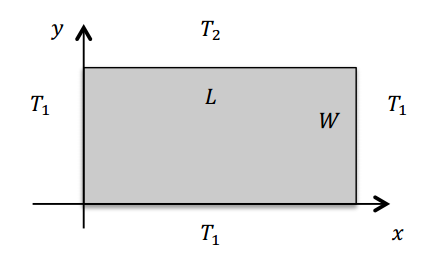
\includegraphics[scale=0.8]{figures/ch3/1}
    \caption{Model of Example3.2.1}
    \label{fig:3:1}
\end{figure}
\end{example}

\begin{solution}
To simplify the solution, use below transformation
$$\theta=\frac{T-T_1}{T_2-T_1}$$
According to heat diffusion equation, the two-dimensional, steady state with no internal heat generation equation is 
$$\frac{\partial^2 T}{\partial x^2}+\frac{\partial^2 T}{\partial y^2}=0$$
the transformed differential equation is then
$$\frac{\partial^2 \theta}{\partial x^2}+\frac{\partial^2 \theta}{\partial y^2}=0$$
Since the equation is second order in both x and y, two boundary conditions are needed for each of the coordinates, they are
$$\theta(0,y)=0,\text{and}  \theta(x,0)=0$$
$$\theta(L,y)=0,\text{and}  \theta(x,W)=1$$
The $\theta(x,y)$ is
$$\theta(x,y)=\frac{2}{\pi}\sum\limits_{i=1}^\infty 
\frac{(-1)^{n+1}+1}{n}\sin{\frac{n\pi x}{L}}
\frac{\sinh{n\pi y/L}}{\sinh{n\pi W/L}}
$$
So that 
$$T(x,y)=(T_2-T_1)\frac{2}{\pi}\sum\limits_{i=1}^\infty 
\frac{(-1)^{n+1}+1}{n}\sin{\frac{n\pi x}{L}}
\frac{\sinh{n\pi y/L}}{\sinh{n\pi W/L}}+T_1
$$
Plot 3D sketch of the temperature distribution in the rectangular is shown as Figure\ref{fig:3:2}
\begin{figure}[h!]
  \centering
    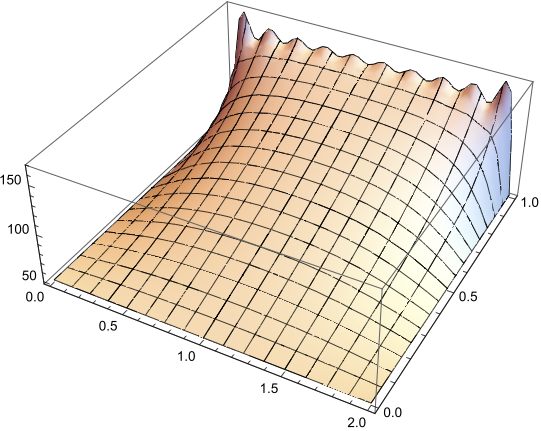
\includegraphics[scale=0.8]{figures/ch3/2}
    \caption{Temperature distribution in square with series method}
    \label{fig:3:2}
\end{figure}

And by fixing $x$ and $y$ separately we can get the temperature distribution $T(1,y)$ as Figure \ref{fig:3:3} and $T(x,0.5)$ as Figure \ref{fig:3:4}
\begin{figure}[h!]
  \begin{minipage}[b]{0.45\linewidth}
  \centering
    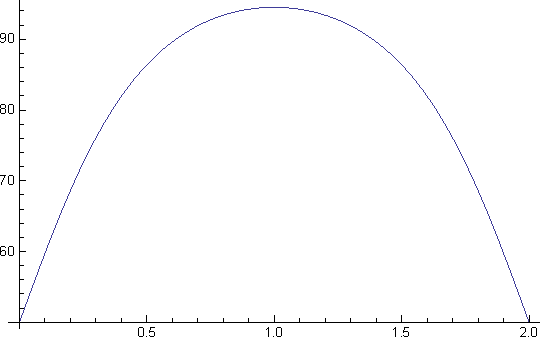
\includegraphics[scale=0.7]{figures/ch3/3}
    \caption{Temperature distribution in square at $x=1$}
    \label{fig:3:3}
\end{minipage}
\hspace{0.5cm}
\begin{minipage}[b]{0.45\linewidth}
  \centering
    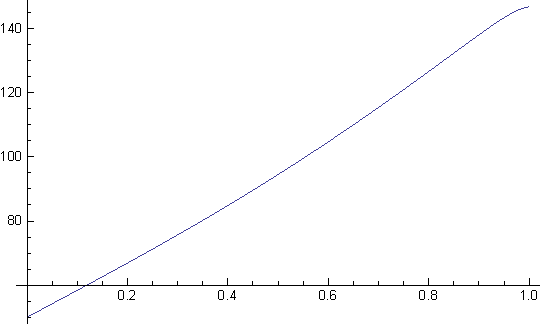
\includegraphics[scale=0.7]{figures/ch3/4}
    \caption{Temperature distribution in square at $y=0.5$}
    \label{fig:3:4}
\end{minipage}
\end{figure}
To calculate the heat flux passing through a unique section line, we use Fourier's equation $q=-kA(\partial T/\partial x\partial y)$ for heat rate at point $(x, y)$. When $y=0$, the heat flux passing through $x$ direction in the square could be represented as

\begin{equation*}
\begin{aligned}
Q&=\int_0^L \! Aq \, \mathrm{d} x|_{y=0} \\
&=2kA(T_2+T_1)\sum\limits_{i=1}^\infty 
\cosh{\frac{(2n-1)\pi y}{2}}\csc{\frac{(2n-1)\pi}{2}}\sin{\frac{(2n-1)\pi x}{2}}|_{y=0}
\\&=8346.27
\end{aligned}
\end{equation*}


\end{solution}




